\documentclass[a4paper,12pt,twoside]{memoir}
\usepackage{listings}
\usepackage[colorlinks]{hyperref}
% Castellano
\usepackage[spanish,es-tabla]{babel}
\selectlanguage{spanish}
\usepackage[utf8]{inputenc}
\usepackage[T1]{fontenc}
\usepackage{lmodern} % Scalable font
\usepackage{microtype}
\usepackage{placeins}
\RequirePackage{booktabs}
\RequirePackage[table]{xcolor}
\RequirePackage{xtab}
\RequirePackage{multirow}

% Links
\PassOptionsToPackage{hyphens}{url}%\usepackage[colorlinks]{hyperref}
\hypersetup{
	allcolors = {red}
}
% Ecuaciones
\usepackage{amsmath}

% Rutas de fichero / paquete
\newcommand{\ruta}[1]{{\sffamily #1}}

% Párrafos
\nonzeroparskip

% Huérfanas y viudas
\widowpenalty100000
\clubpenalty100000

% Imagenes
\usepackage{graphicx}
\newcommand{\imagen}[2]{
	\begin{figure}[!h]
		\centering
		\includegraphics[width=0.9\textwidth]{#1}
		\caption{#2}\label{fig:#1}
	\end{figure}
	\FloatBarrier
}

\newcommand{\imagenflotante}[2]{
	\begin{figure}%[!h]
		\centering
		\includegraphics[width=0.9\textwidth]{#1}
		\caption{#2}\label{fig:#1}
	\end{figure}
}



% El comando \figura nos permite insertar figuras comodamente, y utilizando
% siempre el mismo formato. Los parametros son:
% 1 -> Porcentaje del ancho de página que ocupará la figura (de 0 a 1)
% 2 --> Fichero de la imagen
% 3 --> Texto a pie de imagen
% 4 --> Etiqueta (label) para referencias
% 5 --> Opciones que queramos pasarle al \includegraphics
% 6 --> Opciones de posicionamiento a pasarle a \begin{figure}
\newcommand{\figuraConPosicion}[6]{%
  \setlength{\anchoFloat}{#1\textwidth}%
  \addtolength{\anchoFloat}{-4\fboxsep}%
  \setlength{\anchoFigura}{\anchoFloat}%
  \begin{figure}[#6]
    \begin{center}%
      \Ovalbox{%
        \begin{minipage}{\anchoFloat}%
          \begin{center}%
            \includegraphics[width=\anchoFigura,#5]{#2}%
            \caption{#3}%
            \label{#4}%
          \end{center}%
        \end{minipage}
      }%
    \end{center}%
  \end{figure}%
}

%
% Comando para incluir imágenes en formato apaisado (sin marco).
\newcommand{\figuraApaisadaSinMarco}[5]{%
  \begin{figure}%
    \begin{center}%
    \includegraphics[angle=90,height=#1\textheight,#5]{#2}%
    \caption{#3}%
    \label{#4}%
    \end{center}%
  \end{figure}%
}
% Para las tablas
\newcommand{\otoprule}{\midrule [\heavyrulewidth]}
%
% Nuevo comando para tablas pequeñas (menos de una página).
\newcommand{\tablaSmall}[5]{%
 \begin{table}
  \begin{center}
   \rowcolors {2}{gray!35}{}
   \begin{tabular}{#2}
    \toprule
    #4
    \otoprule
    #5
    \bottomrule
   \end{tabular}
   \caption{#1}
   \label{tabla:#3}
  \end{center}
 \end{table}
}

%
% Nuevo comando para tablas pequeñas (menos de una página).
\newcommand{\tablaSmallSinColores}[5]{%
 \begin{table}[H]
  \begin{center}
   \begin{tabular}{#2}
    \toprule
    #4
    \otoprule
    #5
    \bottomrule
   \end{tabular}
   \caption{#1}
   \label{tabla:#3}
  \end{center}
 \end{table}
}

\newcommand{\tablaApaisadaSmall}[5]{%
\begin{landscape}
  \begin{table}
   \begin{center}
    \rowcolors {2}{gray!35}{}
    \begin{tabular}{#2}
     \toprule
     #4
     \otoprule
     #5
     \bottomrule
    \end{tabular}
    \caption{#1}
    \label{tabla:#3}
   \end{center}
  \end{table}
\end{landscape}
}

%
% Nuevo comando para tablas grandes con cabecera y filas alternas coloreadas en gris.
\newcommand{\tabla}[6]{%
  \begin{center}
    \tablefirsthead{
      \toprule
      #5
      \otoprule
    }
    \tablehead{
      \multicolumn{#3}{l}{\small\sl continúa desde la página anterior}\\
      \toprule
      #5
      \otoprule
    }
    \tabletail{
      \hline
      \multicolumn{#3}{r}{\small\sl continúa en la página siguiente}\\
    }
    \tablelasttail{
      \hline
    }
    \bottomcaption{#1}
    \rowcolors {2}{gray!35}{}
    \begin{xtabular}{#2}
      #6
      \bottomrule
    \end{xtabular}
    \label{tabla:#4}
  \end{center}
}

%
% Nuevo comando para tablas grandes con cabecera.
\newcommand{\tablaSinColores}[6]{%
  \begin{center}
    \tablefirsthead{
      \toprule
      #5
      \otoprule
    }
    \tablehead{
      \multicolumn{#3}{l}{\small\sl continúa desde la página anterior}\\
      \toprule
      #5
      \otoprule
    }
    \tabletail{
      \hline
      \multicolumn{#3}{r}{\small\sl continúa en la página siguiente}\\
    }
    \tablelasttail{
      \hline
    }
    \bottomcaption{#1}
    \begin{xtabular}{#2}
      #6
      \bottomrule
    \end{xtabular}
    \label{tabla:#4}
  \end{center}
}

%
% Nuevo comando para tablas grandes sin cabecera.
\newcommand{\tablaSinCabecera}[5]{%
  \begin{center}
    \tablefirsthead{
      \toprule
    }
    \tablehead{
      \multicolumn{#3}{l}{\small\sl continúa desde la página anterior}\\
      \hline
    }
    \tabletail{
      \hline
      \multicolumn{#3}{r}{\small\sl continúa en la página siguiente}\\
    }
    \tablelasttail{
      \hline
    }
    \bottomcaption{#1}
  \begin{xtabular}{#2}
    #5
   \bottomrule
  \end{xtabular}
  \label{tabla:#4}
  \end{center}
}



\definecolor{cgoLight}{HTML}{EEEEEE}
\definecolor{cgoExtralight}{HTML}{FFFFFF}

%
% Nuevo comando para tablas grandes sin cabecera.
\newcommand{\tablaSinCabeceraConBandas}[5]{%
  \begin{center}
    \tablefirsthead{
      \toprule
    }
    \tablehead{
      \multicolumn{#3}{l}{\small\sl continúa desde la página anterior}\\
      \hline
    }
    \tabletail{
      \hline
      \multicolumn{#3}{r}{\small\sl continúa en la página siguiente}\\
    }
    \tablelasttail{
      \hline
    }
    \bottomcaption{#1}
    \rowcolors[]{1}{cgoExtralight}{cgoLight}

  \begin{xtabular}{#2}
    #5
   \bottomrule
  \end{xtabular}
  \label{tabla:#4}
  \end{center}
}



\graphicspath{ {./img/} }

% Capítulos
\chapterstyle{bianchi}
\newcommand{\capitulo}[2]{
	\setcounter{chapter}{#1}
	\setcounter{section}{0}
	\setcounter{figure}{0}
	\setcounter{table}{0}
	\chapter*{#2}
	\addcontentsline{toc}{chapter}{#2}
	\markboth{#2}{#2}
}

% Apéndices
\renewcommand{\appendixname}{Apéndice}
\renewcommand*\cftappendixname{\appendixname}

\newcommand{\apendice}[1]{
	%\renewcommand{\thechapter}{A}
	\chapter{#1}
}

\renewcommand*\cftappendixname{\appendixname\ }

% Formato de portada
\makeatletter
\usepackage{xcolor}
\newcommand{\tutor}[1]{\def\@tutor{#1}}
\newcommand{\course}[1]{\def\@course{#1}}
\definecolor{cpardoBox}{HTML}{E6E6FF}
\def\maketitle{
  \null
  \thispagestyle{empty}
  % Cabecera ----------------
\noindent
\includegraphics[width=\textwidth]{cabecera}\vspace{1cm}%
  \vfill
  % Título proyecto y escudo informática ----------------
  \colorbox{cpardoBox}{%
    \begin{minipage}{.8\textwidth}
      \vspace{.5cm}\Large
      \begin{center}
      \textbf{TFG del Grado en Ingeniería Informática}\vspace{.6cm}\\
      \textbf{\LARGE\@title{}}
      \end{center}
      \vspace{.2cm}
    \end{minipage}

  }%
  \hfill\begin{minipage}{.20\textwidth}
    
\includegraphics[width=\textwidth]{escudoInfor}
  \end{minipage}
  \vfill
  % Datos de alumno, curso y tutores ------------------
  \begin{center}%
  {%
    \noindent\LARGE
    Presentado por \@author{}\\ 
    en Universidad de Burgos --- \@date{}\\
    Tutores: \@tutor{}\\
  }%
  \end{center}%
  \null
  \cleardoublepage
  }
\makeatother

\newcommand{\nombre}{Gonzalo Murillo Montes} %%% cambio de comando

% Datos de portada
\title{EDVR, super resolución en secuencias de vídeo para su mejora de calidad/restauración}
\author{\nombre}
\tutor{ Dr. Pedro Latorre Carmona y Dr. César Ignacio García Osorio}
\date{\today}

\begin{document}

\maketitle


\newpage\null\thispagestyle{empty}\newpage


%%%%%%%%%%%%%%%%%%%%%%%%%%%%%%%%%%%%%%%%%%%%%%%%%%%%%%%%%%%%%%%%%%%%%%%%%%%%%%%%%%%%%%%%
\thispagestyle{empty}


\noindent
\includegraphics[width=\textwidth]{cabecera}\vspace{1cm}

\noindent D. Pedro Latorre Carmona, y D. César Ignacio García Osorio, profesores del departamento de Ingeniería Infomática, Área de Lenguajes y Sistemas Informáticos.

\noindent Exponen:

\noindent Que el alumno D.Gonzalo Murillo Montes, con DNI 71309704K, ha realizado el Trabajo final de Grado en Ingeniería Informática titulado EDVR, super resolución en secuencias de vídeo para su mejora de calidad/restauración. 

\noindent Y que dicho trabajo ha sido realizado por el alumno bajo la dirección de los que suscriben, en virtud de lo cual se autoriza su presentación y defensa.

\begin{center} %\large
En Burgos, {\large \today}
\end{center}

\vfill\vfill\vfill

% Author and supervisor
\begin{minipage}{0.45\textwidth}
\begin{flushleft} %\large
Vº. Bº. del Tutor:\\[2cm]
D. Pedro Latorre Carmona
\end{flushleft}
\end{minipage}
\hfill
\begin{minipage}{0.45\textwidth}
\begin{flushleft} %\large
Vº. Bº. del co-tutor:\\[2cm]
D. César García Osorio
\end{flushleft}
\end{minipage}
\hfill

\vfill

% para casos con solo un tutor comentar lo anterior
% y descomentar lo siguiente
%Vº. Bº. del Tutor:\\[2cm]
%D. nombre tutor


\newpage\null\thispagestyle{empty}\newpage




\frontmatter

% Abstract en castellano
\renewcommand*\abstractname{Resumen}
\begin{abstract}

La super resolución/restauración de vídeos es una técnica  muy usada hoy en día en diferentes campos de investigación tanto del ámbito industrial, como del de la defensa. Vivimos en una sociedad digital y por lo tanto el aumento de la cantidad de detalles y de calidad en los elementos multimedia son dos características no triviales a las que la super resolución ofrece una gran mejoría.

En este proyecto se aplica una técnica de super resolución de vídeos ganadora del NTIRE (\emph{New Trends in Image Restoration and Enhancement}) challenge 2019, en las categorías dedicadas al vídeo, EDVR (vídeo Restoration with Enhanced Deformable Convolutional Networks). El objetivo es comprobar los resultados de EDVR e implementar vídeos propios para su procesado. Estos vídeos propios serían de gestos y acciones humanas. Para complementar a esta herramienta se ha  desarrollado una interfaz para poder implementar vídeos, poder procesarlos y visualizar los resultados.

\end{abstract}

\renewcommand*\abstractname{Descriptores}
\begin{abstract}
Super resolución, vídeos, deblurring, denoising, deblocking, NITRE (New Trends in Image Restoration and Enhancement) 2019, Python.
\end{abstract}

\clearpage

% Abstract en inglés
\renewcommand*\abstractname{Abstract}
\begin{abstract}

Super resolution/video restoration is a technique widely used nowadays in different research fields, both in the industrial and defense fields. We live in a digital society and therefore the increase in the amount of detail and quality in multimedia elements are two non-trivial features to which super resolution offers a great improvement.

In this project we apply a super resolution video technique winner of the NTIRE (New Trends in Image Restoration and Enhancement) challenge 2019, in the categories dedicated to video, EDVR (video Restoration with Enhanced Deformable Convolutional Networks). The objective is to test the results of EDVR and implement own videos for processing. These own videos would be of human gestures and actions. To complement this tool, an interface has been developed to implement videos, process them and visualize the results.

\end{abstract}

\renewcommand*\abstractname{Keywords}
\begin{abstract}
Super resolution, vídeos, deblurring, denoising, deblocking, NITRE (New Trends in Image Restoration and Enhancement) 2019, Python.
\end{abstract}

\clearpage

% Indices
\tableofcontents

\clearpage

\listoffigures

\clearpage

\mainmatter
\capitulo{1}{Introducción}

Hoy en día vivimos en un mundo basado en la digitalización completa de todos los sectores, y en esta realidad los vídeos tienen un valor muy importante. Todo el mundo tiene en sus manos dispositivos que permiten la adquisición de vídeo, pero no siempre se obtienen los resultados que se desearían. También hay sectores que requieren de gran calidad en los vídeos para diversos fines, militar, seguridad, astronomía, medicina, etc.\
La tecnología ha evolucionado mucho desde la primera vez que se grabó el primer vídeo, allá por 1895 con los hermanos Lumière~\cite{Salas_Murillo_2010}, esta grabación no se puede comparar con ningún  vídeo actual, la super resolución/restauración  ofrece soluciones a todos los casos expuestos, mejorándolos en diversos aspectos y ayudando a su mejor comprensión, calidad y visibilidad. 

 La definición de vídeo es:  tecnología de grabación, procesamiento, almacenamiento, transmisión de imágenes y reconstrucción por medios electrónicos digitales o analógicos de una secuencia de imágenes que representan escenas en movimiento~\cite{wiki:video}. Pero en el contexto en el que nos encontramos reduciremos el término  a una secuencia de imágenes en movimiento. Gracias al Machine Learning, los algoritmos para la restauración de vídeos y super resolución  están  mejorando a pasos agigantados, corrigiendo detalles y mejorando la calidad de los vídeos procesados. 
 
 La super resolución de vídeo permite crear versiones de los vídeos en los que los problemas como el desenfoque, emborronamiento, etc., no existen. Estos problemas afectan de forma directa a métodos posteriores de aprendizaje máquina, como podrían ser los métodos de reconocimiento de acciones humanas.

Una mejora en estos aspectos permitiría aumentar la tasa de acierto de los clasificadores de forma considerable.
 
 Una gran parte de estas implementaciones se basan en obtener información aprovechandose de la redundancia en información intrínseca de imágenes temporalmente contiguas, en secuencias de vídeo. temporalmente contiguos, en estas secuencias de vídeo. EDVR (\emph{Enhanced Deformable Convolutional Networks}) es el modelo usado en este Trabajo de Fin de Grado, se engloba en este grupo y usa Pytorch para lograr mejorarlos. Destaca en los siguientes aspectos.

\begin{itemize}
	\item Super resolución.
	\item Eliminación del emborronamiento.
	\item Reducción de ruido.
	\item Compresión.
\end{itemize}

El funcionamiento básico de EDVR consiste en, partiendo de un  vídeo:

\begin{itemize}
\item Convertirlo en fotogramas.
\item Transformar los fotogramas a baja calidad.
\item Ejecutar el procesado de EDVR.
\item Recomponer el vídeo con los fotogramas procesados. 
\end{itemize}
Para ello también se implementa una interfaz que simplifica el proceso.

\section{Estructura de la memoria}

\begin{itemize}
	\item \textbf{Objetivos del proyecto:} se definen los objetivos generales, técnicos y personales que se persiguen con la realización de este trabajo. 
	\item \textbf{Conceptos teóricos:} se explican los conceptos teóricos que se han manejado en el desarrollo de este proyecto. 
	\item \textbf{Técnicas y herramientas:} se enumeran y explican las distintas técnicas metodológicas y herramientas que se han usado. 
	\item \textbf{Aspectos relevantes del desarrollo del proyecto:} se exponen los problemas que se han afrontado durante el desarrollo del proyecto y las decisiones que se han tomado para solucionarlos. 
	\item \textbf{Trabajo relacionados:} se resume la información encontrada durante la exploración inicial del estado del arte. 
	\item \textbf{Conclusiones y líneas de trabajo futuras:} se exponen las conclusiones generales y personales del proyecto y se enumeran una serie de posibles líneas de trabajo futuras. 
\end{itemize}

\section{Materiales adjuntos}
\begin{itemize}	
	\item \textbf{Anexos:}
	\begin{itemize}
		\item Plan de Proyecto.
		\item Especificación de Requisitos.
		\item Especificación de diseño.
		\item Documentación técnica de programación.
		\item Documentación de usuario.
	\end{itemize}
	\item \textbf{Cuaderno de demostración:} Notebook de Jupyter que contiene el tutorial de instalación junto con una ejecución de prueba de EDVR.
	\item \textbf{Mini conjunto de pruebas:} Parte del conjunto de datos REDS (REalistic and Dynamic Scenes) que contiene 800 imágenes para la ejecución de prueba EDVR, además de parte de los modelos pre-entrenados.
	\item \textbf{Interfaz:} Código y requerimientos para poder usar la interfaz.
\end{itemize}

A la memoria y a todos los demás materiales adjuntos se puede acceder a través del repositorio del proyecto en GitHub: \url{https://github.com/gonmurillo/TFG_EDVR}. 
\capitulo{2}{Objetivos del proyecto}

En este apartado se exponen los objetivos perseguidos con la realización de este trabajo: 


\section{Objetivos generales}

\begin{itemize}
    \item Conseguir la instalación y funcionamiento de EDVR en el equipo de pruebas.
    
    \item Probar a implementar mis propios vídeos en la ejecución de EDVR y comparar resultados.
    
     \item Analizar el impacto de la mejora de estos vídeos sobre casos concretos en los que aparecen gestos y acciones humanas simples.
    
    \item Reducir el tiempo de descarga de datasets y modelos preentrenados necesarios para probar EDVR, para ello se  proporciona un mini conjunto de pruebas.
    
     \item Probar el funcionamiento de un algoritmo de aprendizaje automático para resolver problemas.
     
    \item Investigar sobre distintas técnicas de super resolución de vídeos e imágenes.

    \item Simplificación de la ejecución mediante una interfaz.
    
    \item Comprobar la viabilidad de su uso para vídeos en los que aparecen acciones humanas sencillas como gestos, así como algunas más complejas.
\end{itemize}


\section{Objetivos técnicos}

\begin{itemize}
    \item Aprender  \LaTeX{}, en concreto su uso en herramientas de edición online (Overleaf).
    
    \item Realizar y exponer los resultados de la demostración en un  notebook de Jupyter empleando código Python.
    
    \item Usar la plataforma GitHub para la gestión del proyecto.
    
    \item Aplicar la metodología Scrum en un proyecto real.
    
    \item Profundizar en el funcionamiento de la biblioteca Pytorch y sus capacidades de aprendizaje automático.
    
    \item EDVR ofrece la posibilidad de trabajar con Slurm para el computo distribuido, aprender cómo trabajar con él y sus posibilidades.
    
    \item Aprender a usar PySimpleGUI para dotar a los programas en Python de una interfaz básica pero funcional, con muchas opciones de personalización.
    
    
    
\end{itemize}


\section{Objetivos personales}

\begin{itemize}
    \item Iniciarme en el campo de la investigación.
    \item Explorar técnicas y herramientas del aprendizaje automático y la mejora de vídeos e imágenes.
    \item Familiarizarme con una herramienta como Tmux que facilita el trabajo multi tarea.
    \item Aprender a generar documentación con \LaTeX{}.
    \item Primera puesta en contacto con un desarrollo real.
    
\end{itemize}

\capitulo{3}{Conceptos teóricos}

\section{Aprendizaje automático}

 En inglés \emph{machine learning}, es un campo de la inteligencia artificial cuyo objetivo es desarrollar técnicas y algoritmos que permitan a las máquinas aprender, por si mismos, a través de la experiencia. Sus principales usos del aprendizaje automático son la detección de patrones, reconocimiento de lenguajes, vehículos autónomos, vídeojuegos, y muchas otras áreas. 
    
 Para desarrollar el aprendizaje se usa un modelo matemático basado en datos de entrenamiento para así realizar predicciones o decisiones sin ser programados para hacer estas tareas~\cite{ Zhang2020}.
    
 Dependiendo del modelo de datos que tengan los algoritmos se pueden agrupar en:
 
 \begin{itemize}
 
  \item \textbf{Aprendizaje supervisado:} establece correspondencias entre los datos de entrada y los de las salidas deseadas. Parte de ejemplos resueltos para luego resolver problemas semejantes.
  
  \item \textbf{Aprendizaje no supervisado:} solo usa los datos como entrada sin saber la clase a la que pertenecen dichos datos. Infiere tanto la forma de las agrupaciones de los datos, como la clase a la que pertenecen.
  
  \item \textbf{Aprendizaje semi-supervisado:} es una mezcla entre el aprendizaje supervisado y el no supervisado, hay una pequeña parte de los datos que se saben a qué clase pertenecen y el resto no.
  
  \item \textbf{Aprendizaje por refuerzo:} el algoritmo aprende observando su entorno, los datos de entrada se basan en la retroalimentación de sus acciones, cuando actúan de forma correcta son recompensados, si no, son penalizados.
  
  \item \textbf{Aprendizaje por transferencia:} consiste en utilizar un modelo preentrenado para una tarea y reutilizarlo para resolver una tarea distinta tras algunos pequeños ajustes iniciales. La idea es que las características de bajo nivel que haya aprendido el modelo puedan reutilizarse, aunque tenga que cambiarse como se combina estas para resolver la nueva tarea. 
  
 \end{itemize}

\section{Restauración de vídeos mediante inteligencia artificial}
 La restauración tanto de vídeos como de imágenes actualmente está avanzando exponencialmente demostrando resultados sorprendentes respecto de los obtenidos hace escasamente unos pocos años. La mayoría de técnicas que surgen actualmente se basan en un aprendizaje supervisado usando un par de imágenes una \emph{GROUND-TRUTH}, la imagen ideal que se tiene por referencia y otra \emph{LOW-RESOLUTION}, que es la misma imagen en baja calidad generada por un modelo de degradación como puede ser un sub-muestreo de tipo lineal o vecino más cercano.
 Estas técnicas no acaban de adaptarse completamente a las situaciones reales, ya que estas presentan una complejidad mucho mas pronunciada que la generada por el proceso de submuestreo ~\cite{9359916}.

 Así mismo las técnicas de restauración deben ser capaces de conseguir los resultados intentando ser lo más eficientes en el tiempo empleado y en los recursos consumidos, memoria y energía, siendo ejecutados en hardware común.
 
 La principal diferencia entre la restauración de vídeos e imágenes radica en que los vídeos suponen una complejidad extra, el aspecto temporal, teniendo en cuenta que las imágenes que lo componen están relacionadas entre sí. ~\cite{8746778}.

 Los aspectos en los que se centran los métodos de restauración de vídeos son los siguientes:
 \begin{itemize}

    \item \textbf{Reducción de ruido:} o \emph{denoising} en inglés, consiste en la eliminación de información que corrompe la señal de vídeo debido a problemas en el canal o proceso de adquisición y/o de transmisión.
    \imagen{ruido}{Ruido generado por mala iluminación (Imagen adquirida por el autor)}
        
    \item \textbf{Eliminación del emborronamiento:} proceso de eliminar aspectos borrosos o distorsionados de las imágenes, que se puede deber al movimiento del objeto a capturar o al movimiento en el momento de la captura del dispositivo de grabación. También puede generarse cuando no hay un correcto enfoque de la lente.
    
    \item \textbf{Eliminación de niebla:} mejorar la calidad de una imagen que se encuentre degradada por causas atmosféricas o por partículas en suspensión en el aire que impiden el reconocimiento parcial de la imagen. ~\cite{inproceedings}
    \imagen{dehaze}{Ejemplo de dehazing (Imagen adquirida por el autor).}

    \item \textbf{Super resolución:} técnicas y algoritmos que parten de una imagen con baja resolución y la transforman en una de mayor resolución, obteniendo un número mayor de píxeles donde se recupera la información de los detalles. Existen múltiples clasificaciones y metodos de super resolución, la más típica son:
        \begin{itemize}
           \item \textbf{Multiframe:} técnica de procesado de imágenes que a partir de un conjunto de imágenes, correspondientes a posiciones espaciales diferentes de la cámara genera una sola imagen en alta resolución. El aspecto temporal influye mucho a la hora del procesado de imágenes~\cite{7919264}.
           
            \item \textbf{Single frame:} técnica de procesado de imágenes que a partir de una sola imagen en baja resolución produce una imagen en alta resolución. No se suele usar en la super resolución de vídeos ya que los vídeos suelen presentar mayor complejidad para su super resolución, lo que no quita que haya muchas opciones para elegir. 
        \end{itemize}
        
     \item \textbf{Compresión:} algunos formatos de imagen tienen una compresión por defecto para reducir el tamaño que ocupan y por lo tanto  pueden perder detalles, por eso se usan métodos para recuperar las pérdidas de información ~\cite{Wang_2016_CVPR}.
     
 \end{itemize}
 
\section{Reconocimiento de acciones}
 El reconocimiento de acciones humanas tiene múltiples aplicaciones, pero sobre todo en vigilancia, análisis de contenido e interacciones entre humanos y ordenadores. El reconocimiento debe ser automático tanto de acciones simples como complejas. Una acción es una secuencia de movimientos que puede  comprender varias partes del cuerpo humano.
 
 \subsection{Tipos de acciones}
  Clasificación según el tipo de acción:
 \begin{itemize}
 
 \item \textbf {Acciones simples:} Los llamados gestos o las acciones que no pueden reducirse a otras más sencillas. Negar con la cabeza, saludar, levantar un pie, son ejemplos de este tipo de acciones.   
 
 \item \textbf {Acciones complejas:} Son una combinación de acciones simples.  Andar, correr, dar un salto, entran es esta clasificación.
 
 \item \textbf {Interacciones:} Son las acciones que surgen de la interacción entre grupos reducidos de personas u objetos. Dos personas dándose la mano, o alguien tocando un instrumento.
 
 \item \textbf {Actividades de grupo:} Las acciones que envuelven a un gran número de personas, como un desfile o una calle concurrida.

  \end{itemize}
 Los dos primeros grupos de acciones, simples y complejas son las que han sido más estudiadas y mejores resultados ofrecen. No obstante, recientemente, hay más esfuerzos que se centran en las interacciones y grupos.
 
 En el contexto de la inteligencia artificial, el objetivo consiste en identificar las acciones de un vídeo con otras  previamente identificadas y así asignarle una etiqueta a cada tipo de acción.  El proceso simplificado consiste en la detección de la persona o partes del cuerpo, el seguimiento de las identificaciones  y por último la asignación del tipo de acción, comparando la información obtenida, con sus conocimientos obtenidos mediante el entrenamiento.
 
  \subsection{Clasificación de algoritmos de reconocimiento de acciones}
  
  A la hora de  seleccionar el algoritmo para la clasificación de los gestos o acciones existen una gran variedad de opciones. A continuación se exponen de forma resumida las consideradas más importantes.
  \begin{figure}[!ht]
		\centering
		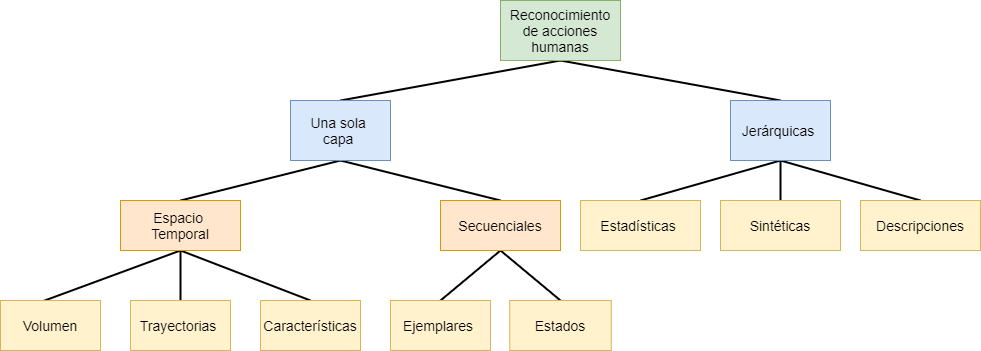
\includegraphics[width=1.1\textwidth]{recoAcciones2}
		\caption{Tipos de algoritmos de reconocimiento de acciones~\cite{article}}\label{1}
	\end{figure}
	\FloatBarrier

         \begin{itemize}
         
            \item \textbf {Una sola capa:} Las acciones se reconocen directamente del vídeo, sin diferenciar en acciones más simples.
            
             \begin{itemize}
             
                \item \textbf {Espacio temporal:} Se basan tanto en la información espacial (imagen 2D), como en la información proporcionada por la variable temporal ($t$), analizando sus interdependencias. Se basan en fijar  unos puntos y estudian su trayectoria en el espacio.
                
                \item \textbf {Secuenciales:} Están diseñados para captar las relaciones temporales de las observaciones, las acciones humanas se integran como una secuencia de observaciones. Una observación se asocia con características extraídas de un conjunto.
                
             \end{itemize}
             
             \item \textbf {Jerárquicas:} Buscan momentos relevantes en las acciones más sencillas, una acción compleja se divide en varias más simples.
             
          \end{itemize}
  

\capitulo{4}{Técnicas y herramientas}

En este apartado se presentan las técnicas metodológicas y las herramientas que se han usado en las distintas fases del desarrollo del proyecto.

\section{Metodología}

    \subsection{Scrum}
    Como se explica más detenidamente en el apartado de Planificación temporal del Apéndice A, para la planificación y desarrollo del proyecto se ha utilizado la metodología ágil Scrum.


\section{Herramientas de la fase de investigación}
    
    \subsection{VPN}
    Virtual Private Network en inglés, es una tecnología de red que permite una extensión de una red de área local estando conectado a Internet. Permite que el ordenador en la red envíe y reciba datos sobre redes compartidas o públicas como si fuera una red privada, con toda la funcionalidad, seguridad y políticas de gestión de una red privada.
        
    Se ha usado FortiClient VPN\footnote{\url{https://www.fortinet.com/support/product-downloads}} para poder conectarme desde casa a la red de la Universidad de Burgos, y poder tener acceso a un equipo que cumpliese los requisitos de EDVR. 
        
    \subsection{Ssh}
    Secure Shell\footnote{\url{https://docs.oracle.com/cd/E36784_01/html/E36870/ssh-1.html}} es un programa que se usa para iniciar sesión en máquinas de manera remota y poder ejecutar comandos. Provee conexiones encriptadas y seguras ente dos hosts  y red no seguras. Las conexiones X11 y los puertos TCP/IP pueden ir en el canal seguro.

    Al iniciar la conexión, lo primero que se requiere es una autentificación, una vez realizado el \emph{login}, nos encontramos ante una terminal normal que se ejecuta en la maquina anfitrión.
    
    \textbf {ssh -X -p 01 gonzalo@10.160.160.120}
    
    \textbf{-X}, que permite X11 forwarding, lo que permite ejecutar aplicaciones graficas de la máquina remota, la aplicación se ejecuta en el host y la interfaz se visualiza en el anfitrión.
    
    \textbf{-p},  indica a el puerto al que conectarse en el host.
    
   
    
    En este proyecto se ha usado para poder conectase a un equipo que pudiese correr EDVR, ya que mi equipo personal no podía ejecutarlo debido a no tener una tarjeta gráfica compatible con CUDA.
    
    \subsection{CUDA}
    Compute Unified Device Architecture es una plataforma de computación en paralelo y un modelo de programación que permite incremento en el rendimiento de computación al aprovechar de la potencia de la unidad de procesamiento de gráficos.
    
    CUDA es un requerimiento  para poder hacer funcionar EDVR, y nos ofrece la posibilidad de usar múltiples GPUs para a la hora de ejecutar los tests y trains.
    
    \subsection{Tmux}
    Es una herramienta de multiplexación de terminales, permitiendo lanzar múltiples terminales en una sola pantalla, pudiendo ser gestionados individualmente. Otra ventaja y la principal razón por la que se ha usado en este trabajo, es la posibilidad de lanzar un script que tarde en ejecutarse y poder cerrar la conexión de ssh. El proceso seguirá ejecutándose mientras la máquina host no se apague, al retomar la conexión podemos volver a el terminal en el que se estaba ejecutando.
    
    Con las circunstancias en las que se a trabajado esto era muy cómodo ya que las desconexiones de la VPN eran relativamente ocasionales.
    
    \subsection{Pytorch}
    Es una biblioteca de Python diseñada para realizar cálculos numéricos haciendo uso los tensores (\emph{arrays} de números que son usados para operaciones), permitiendo su ejecución en GPU para acelerar los cálculos. Es muy utilizada en el campo del \emph{machine learning} y es precisamente por eso que se usa en EDVR. Tiene compatibilidad con CUDA.


\section{Herramientas de la fase de experimentación}
    
    \subsection{Matlab}
    Es una plataforma de programación y cálculo numérico usada para analizar datos, desarrollar algoritmos y crear modelos. Usa su propio lenguaje de programación, M. 
    
    \imagen{pelota}{Ejemplo de imagen extraída de un vídeo de resolución $720\times 1280$ píxeles y la misma imagen procesada por Matlab de resolución $180\times 320$ píxeles}

    En el proyecto se usó inicialmente para transformar las imágenes reduciendo su tamaño mediante submuestreo bicúbico, siendo estas las imágenes que se procesan en EDVR.
    
    A la hora de  implementar la interfaz y automatizar los procesos previos para ejecutar EDVR, en un primer momento se usó una biblioteca para Python que se encargaba de iniciar el Matlab Engine para poder ejecutar el código escrito en matlab. No obstante, finalmente se decidió que la versión final no se iba a usar Matlab ya que es una herramienta de pago y no todo el mundo tiene acceso a ella. En su lugar se usó código en Python para conseguir la misma transformación de las imágenes.

    \subsection{FFmpg}
    Es una colección de software libre que permite grabar, convertir y hacer streaming de audio y vídeo.
    
    Al implementar los vídeos propios y no usar los proporcionados en los datasets, aquí entra FFmpeg. Usamos su funcionalidad para convertir los vídeos en frames con el siguiente comando
    
    \verb|ffmpeg -i name.mp4  -start_number 0 "%08d.png"|
    
    \textbf{-i}: Indica el archivo de entrada.
    
    \textbf{-start\_number}: Indica que el primer frame empiece en el 0 y no en el 1.
    
    \textbf{\%08d.png}: Los archivos de salida empezarán por 8 ceros e irán incrementándose.
    
    La otra función para la que se usa FFmpeg es para convertir los frames procesados en vídeo.
    
    \verb|ffmpeg -framerate 30 -pattern\_type glob -i '*.png'   -c:v libx264|
    
    \verb|-pix\_fmt yuv420p name.mp4|
    
    \textbf{-framerate}: El número de frames por segundo.
    
    \textbf{-pattern\_type}: Ror defecto glob.
    
    \textbf{-i}: Indica los archivos a usar como entrada.
    
    \textbf{-c}: Selecciona el encoder.
    
    \textbf{-pix\_fmt}: El formato de pixels.
    
    A la hora de implementar FFmpeg a la interfaz se opto por usar una biblioteca de Python que implementa FFmpeg en su totalidad, ffmpeg-python. Se usa tanto en la transformación de vídeo a frames, como en su posterior recomposición.\footnote{\url{https://github.com/kkroening/ffmpeg-python}}
    

    \subsection{Jupyter Notebook}
    Es una aplicación web que permite crear documentos con código, ecuaciones, visualizaciones y texto.  Se encuentra incorporado en Anaconda. Se ha usado un notebook totalmente funcional para hacer un pequeña introducción a EDVR así como una demostración de su funcionamiento.


\section{Herramientas de la fase de desarrollo}

    \subsection{PySimpleGUI}
    Es un paquete de Python que permite  crear interfaces para programas en Python. Es muy sencillo de usar se crea una ventana y puedes añadir elementos sin apenas código. Ofrecen en su web y Github \footnote{\url{https://github.com/PySimpleGUI/PySimpleGUI}} gran cantidad de código listo para usarse para demostrar su funcionamiento, cambiar pequeños aspectos y dar ideas. Casi hay una implementación para todas las ideas que se te ocurran.
    
    \subsection{Cv2}
    OpenCV es una biblioteca multiplataforma de visión artificial, aunque en el proyecto no se usa para eso, sino para lo mismo que se usaba Matlab, transformar las imágenes que se extraen de los vídeos, a las mismas redimensionadas y en baja calidad.
    
    GaussianBlurr para reducir el ruido y detalle.
    
    Resize con bicubic interpolation para reducir la imagen. 

    \subsection{Python-VLC}
    VLC\footnote{\url{https://www.vídeolan.org/vlc/index.es.html}} es un reproductor multimedia libre y de código abierto multiplataforma y un framework que reproduce la mayoría de los archivos multimedia.
    
    Se usa el módulo de Python para reproducir el vídeo generado por EDVR dentro de la interfaz. Para poder usar el módulo se requiere tener instalado VLC en el equipo.


\section{Otras herramientas}

    \subsection{Google Drive}
    Es un servicio de alojamiento de archivos de Google. Uno de los dataset que usa EDVR está alojado en esta plataforma  y también se ha usado como intermediario para transferir archivos entre mi equipo y el equipo propiedad de la Universidad de Burgos.
    
    \subsection{Overleaf}
    En un  editor colaborativo de \LaTeX{} online para la generación de la presente memoria y anexos.
    
    \subsection{GitHub}    
    GitHub es una plataforma de desarrollo colaborativo utilizado para alojar proyectos y utilizar el sistema de control de versiones Git.



\capitulo{5}{Aspectos relevantes del desarrollo del proyecto}

    Antes de hablar y profundizar sobre EDVR, el modelo implementado en el Trabajo de fin de grado, se explicará el concurso del que fue ganador en las categorías de vídeo, NTIRE Challenge 2019.
    
    \section{NTIRE Challenge video 2019}

   NTIRE (New Trends in Image Restoration and Enhancement) challenge es un workshop que lleva realizándose desde 2017. El objetivo que ha tenido y tiene siempre es presentar los avances y tendencias en el campo de la restauración y mejora de imágenes y vídeos. También pretende servir como punto de encuentro entre empresas y desarrolladores para lograr colaboraciones. 

    Siempre distingue entre dos tipos generales de retos, que son problemas expuestos por los organizadores que plantean dificultades de ejecución, y cada uno de estos retos se divide a su vez en otros más especializados.
    \begin{itemize}
    \item Retos de imágenes
    \item Retos de vídeos
    \end{itemize}
    
    Por la naturaleza del trabajo solo nos centraremos en los retos del 2019 en la categoría de vídeos, los cuales fueron ganados por EDVR.
    
    \subsection {Challenge on video Super-Resolution ~\cite{Nah_2019_CVPR_Workshops}}
        Los objetivos de este reto son: impulsar las técnicas actuales de super resolución, comparar diferentes soluciones, promover el uso del dataset REDS y promover retos más difíciles para la super resolución de vídeos.
        
        \begin{itemize}
        \item\textbf {\emph{Track 1 clean}} Versión adaptada para métodos comunes de super resolución, ya que emplea degradación mediante submuestreo bicúbico de factor 4, las imágenes tienen un tamaño 4 veces menor al original.
        
        \item\textbf {\emph{Track 2 blur }} Versión más complicada, ya que incluye emborronamientos debido a objetos en movimiento y a movimiento de cámaras.  Son vídeos más acordes con la realidad.
        \end{itemize}
        
    \subsection {Challenge on video Deblurring ~\cite{NITRE_CVD}}
        Los objetivos de este reto son: impulsar las técnicas actuales de eliminación de emborronamiento, comparar diferentes soluciones, promover el uso del dataset REDS y promover retos más difíciles para el desemborronamiento de vídeos.  

        \begin{itemize}
        \item\textbf {Track 1 clean} Versión adaptada para métodos comunes para la eliminación de emborronamientos de vídeos. Los emborronamientos son los propios del movimiento de la cámara y de los objetos en movimiento.
        
        \item\textbf {Track 2 compression artifacts} Se incluye los mismos problemas que el apartado anterior pero ahora los vídeos presentan compresión del 60\%.
        \end{itemize}

\section{REDS}
    REalistic and Dynamic Scenes~\cite{Nah_2019_CVPR_Workshops_REDS}, es el dataset oficial del NITRE Challenge vídeo y aspira a ser un referente en el aparatado de la super resolución y desemborronamiento de vídeos.
    
    Compuesto por 30.000 imágenes extraídas de vídeos grabados por el equipo que lo desarrolla. La resolución se asemeja a los estándares actuales siendo de $720\times 1280$. La manera de crear las imágenes borrosas naturales consiste en aumentar los fotogramas por segundo (fps), y usar una red neuronal convolucional (CNN) para rellenar los detalles perdidos.
    
    El dataset está dividido en 5 apartados:
        \begin{itemize}
        \item\textbf {Original} También conocido como GT (Ground Truth). Se usan principalmente como imágenes de referencia con que comparar  las imágenes obtenidas por los métodos de super resolución/restauración.
        \item\textbf {Borroso.} 
        \item\textbf {Borroso y comprimido.} 
        \item\textbf {Baja resolución.} 
        \item\textbf {Borroso y baja resolución.} 
        \end{itemize}
    El dataset puede ser descargado aquí: \url{https://seungjunnah.github.io/Datasets/reds.html}

\section{Vimeo 90K}
    Es un dataset desarrollado mediante la selección de vídeos de la plataforma Vimeo para un modelo de mejora de vídeos basado en la estimación de los movimientos~\cite{xue2019video}. Una red neuronal con un componente de entrenamiento  para la predicción de movimiento y el procesamiento de vídeo.
    
    Formado por casi 90.000 clips de vídeos con multitud de escenarios y diversidad. Creado específicamente para la restauración de vídeos. Todos los clips tienen un tamaño estándar de $448\times 256$ píxeles.
    
    El dataset puede ser descargado aquí: \url{http://toflow.csail.mit.edu/}
    
\section{Estructura y funcionamiento de EDVR}    

    EDVR ~\cite{wang2019edvr} es el acrónimo de Enhanced Deformable convolutions Video Restoration, es una herramienta contenida en BasicSR (\emph{Basic Super Restoration}), un proyecto OpenSource de restauración para imágenes y vídeos, que también contiene a EDSR (\emph{Enhanced Deep Residual Networks}), RCAN (\emph{Residual Channel Attention Networks}), SRResNet (\emph{Super Resolution ResNet}), SRGAN (\emph{Super Resolution Generative Adversarial Network}), ESRGAN (\emph{Enhanced Super-Resolution Generative Adversarial Networks}), StyleGAN2 (\emph{Style Generative Adversarial Network 2}) y DFDNet (\emph{Dictionary Feature Transfer Net}).
    
    EDVR está basado en dos módulos fundamentales que son los responsables de la eficiencia del método. Un módulo de alineamiento de convoluciones PCD (\emph{Pyramid, Cascading and Deformable}) y un módulo de fusión TSA (\emph{Temporal and Spatial Attention}). Partiendo de $2N+1$ fotogramas en baja calidad, denominamos  $I_t$ al fotograma central  y el resto se denominan fotogramas adyacentes. El objetivo de la restauración de vídeo es estimar una imagen de alta calidad que se asemeje a la imagen de referencia, GT.

    \imagen{frameworkEDVR}{Estructura de funcionamiento interno EDVR~\cite{wang2019edvr}}
    
    Previo a la aplicación de PCD y TSA, se ofrece la posibilidad de aplicar un módulo de  eliminación del emborronado a las imágenes de entrada para mejorar el alineamiento de características.
    
    \subsection {PCD}
        Acrónimo de \emph{Pyramid, Cascading and Deformable convolution} inspirado por TDAN (\emph {Temporally Deformable Alignment Network}) ~\cite{tian2018tdan}, que también usa el alineamiento mediante convoluciones deformables(operaciones de pequeñas agrupaciones de píxeles para puntuar las características de la imagen) para los alinear las características de los fotogramas adyacentes. 

        \imagen{PCD}{Módulo PCD \emph{Pyramid, Cascading and Deformable convolution} de EDVR~\cite{wang2019edvr}}
    
        Partiendo de un núcleo de convolución deformable de $K$ posiciones de muestreo, se denota $w_k$  y  $p_k$ al peso y a las compensaciones preestablecidas para cada posición $K$. Las características alineadas  en cada posición  $p_0$ se obtienen por:
        \begin{equation}\label{12}
            F^a_{t+i} (p_0) = \sum^K_{k=1} w_k * F_{t+1}(p_0 + p_k +\Delta p_k) * \Delta m_k
        \end{equation}
      Donde * es el operador de convolución y la compensación aprendible $\Delta p_k $ y el escalar de modulación $\Delta m_k $ son predichos concatenando características del fotograma central y los adyacentes.
        
         \begin{equation}\label{27}
          \Delta P_{t+i} = f([F_{t+i}, F_t]), i \in [-N:+N]
        \end{equation}
        
        \noindent $f$ es una función general de varias capas de convolución y  [·, ·] es la concatenación.
        La principal diferencia es el modo de hacerlo, se usa una estructura piramidal que primero se centra en la alineación de las características de los detalles de manera amplia, para luego aumentar la perspectiva y compensar de manera precisa los movimientos.
        
        Para generar la característica $F^l_{t+i}$ en los niveles se usan filtros de convolución estriados(mayor desplazamiento de las agrupaciones de píxeles) para reducir la muestra de las características en $l-1$ nivel de la pirámide en un factor de 2, obteniendo pirámides de representación de características de $L$ niveles. En los niveles los desplazamientos y el lineamiento de características también son predichas con los desplazamientos x2 y las características del nivel $l+1$.

        \begin{equation}\label{39}
          \Delta P_{t+i} = f([F_{t+i}, F_t], (\Delta P^{l+1}_{t+i})^{\uparrow 2})
          (F^a_{t+1})^l = g(DCon(F^l_{t+i},\Delta P^l_{t+i}), ((F^a_{t+i})^{l+1})^{\uparrow 2})
        \end{equation}

        $(.)^{\uparrow s}$ es el factor de escalado, DConv es la convolución deformable de la primera fórmula y g es  una función general con varias capas de convolución. 
        EDVR usa una pirámide de 3 niveles.
         Adicionalmente se realiza una convolución deformable que mejora la alineación.

    \subsection {TSA}
        Acrónimo de \emph{Temporal and Spatial Attention} ayuda al añadido de información a través de las características alineadas. Para eso se usa la fusión con atención temporal(proceso para centrarse en los aspectos relevantes de una secuencia) para calcular la correlación entre el fotograma central y los adyacentes. Estos cálculos se usan para saber cuáles son las mejores características que se usaran para reconstruir el fotograma central. Tras esto se aplica la atención espacial para asignar pesos a las ubicaciones en cada canal para compartir información entre canales.
        
        \imagen{TSA}{Módulo TSA \emph{Temporal and Spatial Attention} de EDVR~\cite{wang2019edvr}}
    
        Para cada fotograma la distancia de similitud $h$ se calcula con:
        \begin{equation}\label{48}
        \tilde{F}^a_{t+i} = F^a_{t+i} \odot h(F^a_{t+i}, F^a_t)
        F_{fusion} = Conv(\tilde{F}^a_{t-N}, \cdot\cdot\cdot, \tilde{F}^a_{t},\cdot\cdot\cdot, \tilde{F}^a_{t+N} )
        \end{equation}
        
        Donde $\odot $  y  [·, ·, ·] son la multiplicación elemento a elemento y la concatenación respectivamente.
        
        Se usa un modelo de pirámide para lograr mayor atención a los detalles, siendo las detalles fusionados mediante sumas y  multiplicaciones.
        
    \subsection{Modo Predeblur}    
    
        Para mejorar los resultados, especialmente en entradas muy borrosas o distorsionadas, se emplea una restauración en dos etapas para mejorar el rendimiento, siendo la primera etapa la descrita hasta ahora. La segunda etapa consiste en una red similar a EDVR, pero menos profunda, que se conecta en cascada para refinar las imágenes de salida de la primera etapa. Elimina el desenfoque de movimiento que no se trata en la primera etapa y mitiga la incoherencia entre las imágenes de salida.

\section{Problemas en el desarrollo}   
    
    \subsection {Incompatibilidad}
    EDVR tiene unos requisitos que han de cumplirse para poder ejecutarlo.
     \begin{itemize}
        \item Una versión de Python igual o superior a la 3.7, recomendando usar Anaconda o Miniconda.
        \item Versión de PyTorch igual o superior a la 1,7.
        \item Tarjeta gráfica de la marca NVIDIA compatible con CUDA.
    \end{itemize}
    Todo esto en el sistema operativo Ubuntu, aunque se recalca que debería poder funcionar en Windows, aunque no está comprobado.

    Mi equipo consiste en un ordenador portátil con sistema operativo Windows, lo cual hubiese sido una limitación y un reto a la vez, pudiendo intentar probar la compatibilidad entre Windows y EDVR, y una tarjeta gráfica NVIDIA GeForce GTX 1650, que en principio no debería generar problemas. Pero antes de probar a instalar nada comprobé en la página web de NVIDIA las tarjetas gráficas compatibles\href{https://developer.nvidia.com/cuda-gpus}. Mi tarjeta gráfica no estaba en la lista, por lo que no podía usar mi equipo para el desarrollo del Trabajo de fin de grado.

    En su lugar el departamento de Ingeniería Informática me permitió el acceso remoto a una máquina que cumplía los requisitos y se ejecutaba en Ubuntu. Es en esta máquina donde se han realizado todas las ejecuciones y pruebas. Para acceder a la máquina se uso una VPN y el comando Ssh. 
    
    \subsection {Datasets}
    Ya se han expuesto los dos datasets que se usan junto a EDVR, REDS y Vimeo 90K. Vimeo 90K no presenta ningún problema para su descarga, más allá de lo pesado que es, 82 GBs comprimidos.
    
    En cambio, REDS pese a no ocupar comprimido mucho más, 98,5 gigas, presenta muchas más complicaciones al descargarlo. Está ubicado en Google Drive y dividido en 14 carpetas, las cuales se descargan individualmente, el problema es que, en Drive, por ser archivos pesados los bloquea temporalmente si mucha gente accede a ellos, estos bloqueos según mi experiencia pueden durar hasta 24 horas, por lo que descargar las 14 carpetas lleva mucho tiempo.

    \subsection {Ejecución}
    Los modelos pre-entrenados se identifican con los datasets, las imágenes tipo REDS ($720\times 1280$ píxeles) con los pretarined models de REDS e igual con las imágenes tipo Vimeo 90K ($448\times 256$ píxeles). Ejemplos de dos de los modelos pre-entrenados:
    
    \textbf{EDVR\_L\_deblurcomp\_REDS\_oficial\-0e988e5c.pth}
    
    \textbf{EDVR\_L\_x4\_SR\_Vimeo90K\_official\-162b54e4.pth}
    
    De la misma manera si se ejecuta el módulo pre eliminación del emborronamiento  también hay que usar los pretarined models que corresponden. Para el caso REDS, en la interfaz se usan dos pretarined models, y dependiendo de si se usa o no este módulo  se usa uno u otro.
    
    \textbf{EDVR\_L\_x4\_{\color{red} SRblur}\_REDS\_official\-983d7b8e.pth} con pre eliminación de emborronado.
    
    \textbf{EDVR\_L\_x4\_{\color{red} SR}\_REDS\_officia\l-9f5f5039.pth} sin pre eliminación de emborronado.
    
    Si se usa el modelo pre entrenado que no se corresponde con el modelo usado, a la hora de ejecutar EDVR saltarán errores que no permitirán su ejecución.
    
    \begin{verbatim}
    021-04-26 09:56:21,908 INFO: Loading EDVR model from
    experiments/pretrained_models/EDVR/
    EDVR_L_x4_SRblur_REDS_official-983d7b8e.pth.
    Traceback (most recent call last):
      File "basicsr/test.py", line 58, in <module>
        main()
      File "basicsr/test.py", line 45, in main
        model = create_model(opt)
      File "/home/edvr/edvr/BasicSR/basicsr/models/
      __init__.py", line 38, in create_model
        model = model_cls(opt)
      File "/home/edvr/edvr/BasicSR/basicsr/models/
      edvr_model.py",line 17, in __init__
        super(EDVRModel, self).__init__(opt)
      File "/home/edvr/edvr/BasicSR/basicsr/models/
      sr_model.py", line 30, in __init__
        self.load_network(self.net_g, load_path,
      File "/home/edvr/edvr/BasicSR/basicsr/models/
      base_model.py", line 262, in load_network
        net.load_state_dict(load_net, strict=strict)
      File "/home/edvr/anaconda3/lib/python3.8/
      site-packages/torch/nn/modules/module.py",
      line 1051, in load_state_dict raise
      RuntimeError('Error(s) in loading state_dict for 
      {}:\n\t{}'.format(
    RuntimeError: Error(s) in loading state_dict for 
    EDVR: size mismatch for fusion.feat_fusion.weight:
    copying a param with shape torch.Size([128, 640,
    1, 1]) from checkpoint, the shape in current model 
    is torch.Size([128, 896, 1, 1]).
    	size mismatch for fusion.spatial_attn1.weight:
    	copying a param with shape torch.Size(
    	[128, 640, 1, 1]) from checkpoint, the shape
    	in current model is torch.Size([128, 896, 1, 1]).
    \end{verbatim}
    Ejemplo de un error al ejecutar EDVR con una resolución de imagen que no se corresponde a la REDS.
    
    \subsection {Programa sustitutivo de Matlab}
    Como ya se ha explicado anteriormente, EDVR requiere una imagen de baja resolución como entrada. Para poder ejecutar el dataset Vimeo 90K es necesario generar las imágenes en baja resolución a partir de las imágenes originales. Los desarrolladores proveen un script de Matlab para lograr esto. En la fase de investigación y pruebas esto no genera ningún inconveniente ya que tengo acceso a una licencia de estudiante de Matlab. A la hora de implementar la interfaz usar Matlab para esta tarea no es viable, ya que es una opción que no todo el  mundo tiene acceso, por lo que se empezó a buscar diferentes alternativas.

    Como primera aproximación se decidió habilitar la comunicación entre Matlab y Python permitiendo ejecutar el script de Matlab en el código de Python, funciona, pero no resuelve la dependencia de Matlab.

    Como segunda opción se probó con la biblioteca de FFmpeg para Python ya que se usa para convertir los vídeos a fotogramas y los fotogramas a vídeos. La transformación se hacía cambiando la resolución a 180x320 con una interpolación bicubica. Tras una ejecución de EDVR este era el resultado \ref{fig:ffmpeg}.

    \imagen{ffmpeg}{Imagen procesada por EDVR, la imagen de entrada fue obtenida con FFmpeg para Python}
    
    Es bastante evidente por qué no se continuó con esta opción, se genera una anomalía ajena al vídeo original. Analizando en retrospectiva, seguramente fuese un problema que pudiese haber sido resuelto. Ya que más adelante se encuentra un problema similar con otra opción, pero se consiguió resolver.

    La siguiente opción que se implemento fue usar la biblioteca Cv2, esta fue finalmente la opción seleccionada. Hay que fijarse en la siguiente línea de código  para explicar las diferentes versiones que se probaron hasta obtener un resultado optimo con EDVR.

    \texttt{hr\_img = cv2.GaussianBlur(hr\_img, (0, 0), 1, 1)}

    Esta línea se encarga de emborronar una imagen, dependiendo de los dos últimos valores se emborronará más o menos. Se hicieron las siguientes pruebas:

    \imagen{gb2}{Imagen procesada por EDVR, la imagen de entrada fue obtenida con Cv2 y gausianblur de valor 1}
    
    Como se observa en la Figura \ref{fig:gb2} los resultados no son claros y en la secuencia de vídeo reconstruida se observa aún más.
    
     \texttt{hr\_img = cv2.GaussianBlur(hr\_img, (0, 0), 3, 3)}

    \imagen{gb3}{Imagen procesada por EDVR, la imagen de entrada fue obtenida con Cv2 y gausianblur de valor 3}
    
    En esta Figura \ref{fig:gb3} se puede observar que el resultado no es correcto tampoco ya que parece que estuviese desenfocada.

     \texttt{hr\_img = cv2.GaussianBlur(hr\_img, (0, 0), 4, 4)}

    \imagen{gb4}{Imagen procesada por EDVR, la imagen de entrada fue obtenida con Cv2 y gausianblur de valor 4}
    
    La Figura \ref{fig:gb4} aun se nota más desenfocada.
    
     \texttt{hr\_img = cv2.GaussianBlur(hr\_img, (0, 0), 0.25, 0.25)}

    \imagen{gb0,25}{Imagen procesada por EDVR, la imagen de entrada fue obtenida con Cv2 y gausianblur de valor 0.25}
    
    La Figura \ref{fig:gb0,25} es probablemente la peor de todas las imágenes mostradas hasta ahora, aparecen las mismas anomalías que había en la versión de FFmpeg y la imagen no obtiene ninguna mejora, solo empeora.  
    
     \texttt{hr\_img = cv2.GaussianBlur(hrº\_img, (0, 0), 2, 2)}

    \imagen{gb1}{Imagen procesada por EDVR, la imagen de entrada fue obtenida con Cv2 y gausianblur de valor 2}
    
    La Figura \ref{fig:gb1} es la versión final, en comparación con el resto de las pruebas sí que genera buenos resultados al procesarse con EDVR.
    
    
\section{Desarrollo de la interfaz}   

    A continuación, se exponen el proceso y decisiones que se tomaron en el desarrollo de la interfaz que integra a EDVR. Todo el desarrollo está basado en PySimpleGUI.
    
    Este proyecto es mi primera toma de contacto con el desarrollo de interfaces, pero pese a que en principio ser esta una tarea que se me antojaba complicada, fue todo lo contrario, gracias a la herramienta que se decidó usar, PySimleGUI.  Ya que es muy intuitiva e incorpora en su GitHub multitud de mini proyectos con ejemplos de lo que se puede conseguir usándola correctamente ~\cite{PySimpleGUI}.
    
    Desde el principio tenía muy claro como quería que la interfaz se viese y los resultados finales no distan mucho de esta planificación.
    
    \imagen{todo}{Conjunto de prototipado de la interfaz para EDVR}\label{todo}
     
    Para demostrar cómo funciona una ventana de PySimpleGUI, se usará el código de la primera ventana de la interfaz.
    
    Lo primero consiste en importar la biblioteca con el nombre de sg, como es indicado por sus desarrolladores. 
    
    \begin{lstlisting}[language=python]
    import PySimpleGUI as sg
    \end{lstlisting}
    
    A continuación, hay que definir como se verá la distribución de la ventana, cada línea dentro de la palabra clave layout será una línea en la interfaz. Es aquí donde empiezan a usarse los Widgets, que son los elementos que se pueden usar en la interfaz Text texto, Input insertar texto, Button botón, etc. Cabe destacar el uso de la expresión key='-xxxxxx-', las xxxx representan el nombre con el que se hace referencia a ese Widget para más tarde modificarlo.
    
    \begin{verbatim}
    layout = [ [sg.Text('Recuerda que solo puede procesar 
                vídeos 720 x 1280 o viceversa')],
              [sg.Text('Elige un vídeo para porcesar')],
              [sg.Input(size=(50,1), key='-OUT-')],
              [sg.Button('Buscar')],
              [sg.Checkbox("¿Quieres usar Predeblur?',
                key='-IN-')],
              [sg.Button('Comenzar'),sg.Button('Exit')] ]
    \end{verbatim}
    
    Hasta ahora solo se ha diseñado la ventana, con esta línea se crea la ventana.
    \begin{lstlisting}[language=python]
    window = sg.Window('EDVR UI', layout)
    \end{lstlisting}
    
    
    
    
    En este último apartado se manejan los eventos las actualizaciones de la ventana y las llamadas a otros métodos o ventanas.
    \begin{verbatim}
    while True: 
            event, values = window.read()
            print(event, values)
            if event in (None, 'Exit'):
                break
            if event == 'Buscar':
                path=sg.popup_get_file('Selecciona un vídeo')
                window['-OUT-'].update(path)
                
            if event == 'Comenzar':
                predb = values['-IN-']
                path_v = values['-OUT-']
                ejecucion(path_v,predb)
        window.close()
    \end{verbatim}
    
    
    La interfaz es sencilla pero funcional, la primera pantalla que nos encontramos contiene las dos primeras pantallas del prototipado \ref{todo}. Aquí se puede poner la ruta al vídeo o  buscar el vídeo en el explorador de carpetas. También se incluye una casilla de verificación para decidir si se usa el modo que elimina más eficazmente el emborronamiento.
    
   \imagen{f1}{Primera pantalla de la interfaz, en la que se selecciona el vídeo y la opción de usar el módulo de eliminación de emborronamiento}
   
   	\begin{figure}[!h]
		\centering
		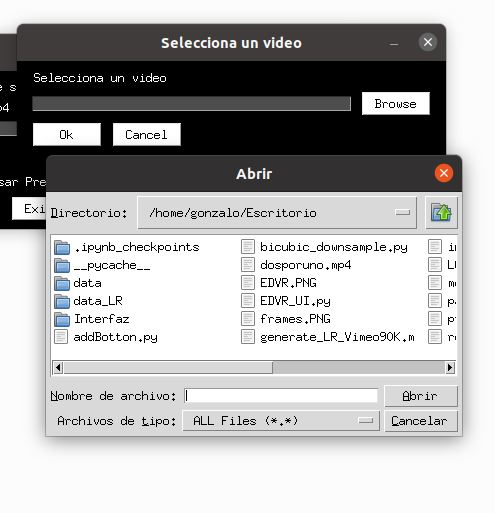
\includegraphics[width=0.8\textwidth]{2}
		\caption{Explorador de archivos para seleccionar el vídeo si no se sabe el \emph{path}}\label{explo}
	\end{figure}

   
   Cuando se hace clic en comenzar, salta una nueva pantalla, se hace clic en generar y empieza la ejecución, el primer paso consiste en convertir el vídeo a fotogramas, cuando la tarea se completa, tardando más cuanto más largo sea el vídeo, salta a la siguiente actualizando el texto y el progreso. 
   
    \imagen{f5}{Barra de referencia para informar de por que parte del procesamiento del vídeo se halla el usuario}
   
   El apartado que más tiempo tarda es el procesado por EDVR, que depende tanto de la duración del vídeo como de la potencia de la máquina que lo esté ejecutando.

    Una vez que acaba todo el proceso se añade un botón y una pregunta que indica si se quiere reproducir el vídeo obtenido mediante el procesamiento.

    \imagen{4}{Reproductor de vídeo}
    
    
\section{Ejemplos de ejecuciones} 

A continuación, se mostrarán algunos ejemplos tanto de vídeos propios procesados por EDVR y ejemplos de los \emph{datasets} usados para el NTIRE Challenge.

  \imagen{pelotaProce}{Primer vídeo propio procesado por EDVR, se observa una pelota cayendo, la imagen de la derecha es la procesada por EDVR.(Imagen adquirida por el autor) }
  
Como se puede observar en la Figura \ref{fig:pelotaProce}, la resolución es mucho mayor, y la calidad es buena. También es muy reseñable la eliminación de las líneas de movimiento alrededor de la pelota.

\imagen{noDedof}{Vídeo en el que se muestra el gesto de negación con el dedo, la imagen de la derecha es la procesada por EDVR. }

En la Figura \ref{fig:noDedof}, las imágenes han sido ampliadas. Como observación general se observa que la imagen izquierda está más pixelada y con menos detalles. En la apliación se muestra el detalle del dedo en movimiento, en la izquierda se observan borrones de movimiento, y en la derecha EDVR ha reconstruido la imagen disminuyendo el emborronamiento, el dedo sigue siendo un poco más grande de lo normal, pero mejora la identificación de la forma básica de un dedo.

Este resultado es muy importante ya que ejemplifica uno de los objetivos del proyecto, ya que aumenta la mejora potencial de la tasa de acierto de métodos automáticos de reconocimiento de gestos y acciones.

\imagen{siCabezaf}{Vídeo en el que se muestra el gesto de afirmación con la cabeza, la imagen de la derecha es la procesada por EDVR.}

La Figura \ref{fig:siCabezaf} muestra el ejemplo de un caso en el que el resultado obtenido no es del todo bueno, en el recuadro de la cara se observa que EDVR no ha procesado bien los movimientos verticales de la cabeza, en la fase de fusionado de imágenes. Pero en contraposición el recuadro de abajo con el dibujo de la camiseta si que se observa bastante mejoría.

\imagen{salto}{Vídeo en el que se muestra el un salto, la imagen de la derecha es la procesada por EDVR.}
En la Figura \ref{fig:salto} se muestra un gesto complejo, ya que el salto es un conjunto de gestos simples. Se muestra el fotograma en medio del aire, en la imagen de la derecha se puede observar mayor calidad con el mismo zoom, las zapatillas se ven mucho menos pixeladas.

\imagen{saltomal}{Captura del vídeo procesado por EDVR en un salto con el modo predeblur.}

En la Figura \ref{fig:saltomal} aparece el mismo fotograma que en la comparación anterior, como se observa el resultado es malo, ya que la figura esta distorsionada, como se observa en el recuadro rojo con la zapatilla. Esto es resultado de usar el modo predeblur cuando no hay emborronamiento. Por lo recomiendo usar solo este modo cuando el  emborronamiento sea abundante.

\begin{figure}[!h]
		\centering
		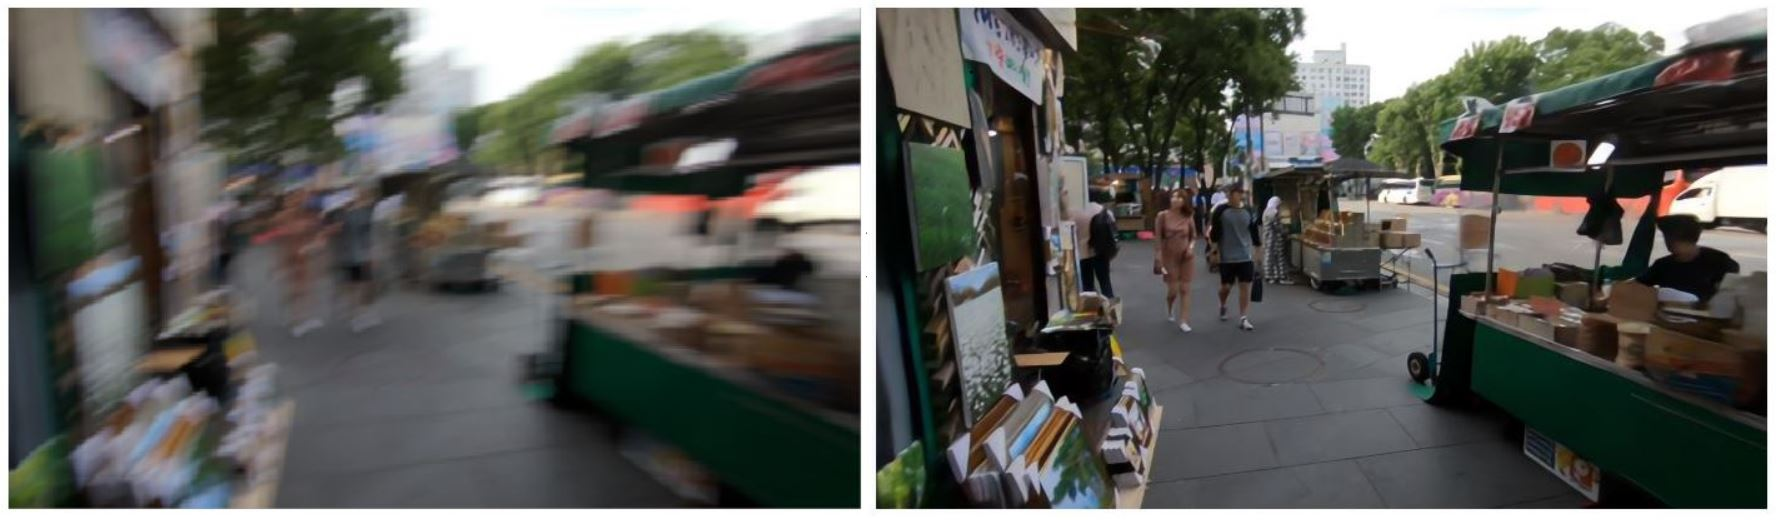
\includegraphics[width=1.1\textwidth]{reds}
		\caption{Vídeo obtenido de REDS, muestra una imagen de un mercado, la imagen de la derecha es la procesada por EDVR~\cite{wang2019edvr}.}\label{5}
	\end{figure}
	\FloatBarrier


Los resultados de la Figura \ref{5} son buenos, lo que muestra la potencia del método en cuanto a su capacidad para mejorar la calidad de los vídeos, también he de decir que el algoritmo está entrenado con imágenes muy parecidas y por eso ofrece mejores resultados que los obtenidos por mí.

\begin{figure}[!h]
		\centering
		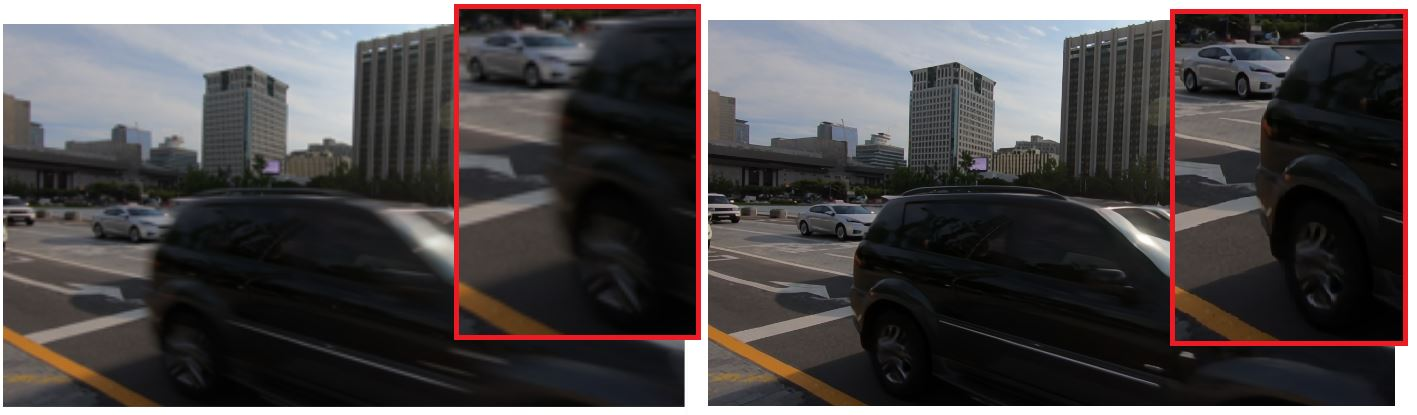
\includegraphics[width=1.1\textwidth]{reds2}
		\caption{Vídeo obtenido de REDS, muestra una imagen de una carretera, la imagen de la derecha es la procesada por EDVR~\cite{wang2019edvr}.}\label{10}
	\end{figure}
	\FloatBarrier

La Figura \ref{10} muestra otra imagen de REDS, esta vez no está tan emborronada, pero también se aprecia muy bien la mejora, solo hay que fijarse en el recuadro rojo que muestra la trasera del coche, como toda la distorsión desaparece y todo está mucho más definido.





\capitulo{6}{Trabajos relacionados}

Para la realización de este proyecto se realizó una exploración inicial del estado del arte de la super resolución y restauración tanto de vídeos e imágenes. En este apartado se exponen algunos artículos más relevantes y aquellos que se centran en técnicas no tan parecidas a EDVR.

\section{WDVR}  
Wide-activated 3D convolutional network for vídeo Restoration \cite{9025696}, centrándose en la restauración  en tres dimensiones: espacial, temporal y canal. Lo normal es que los modelos de super resolución se centren en los aspectos espaciotemporales.

Este método se caracteriza por su eficacia con hardware limitado y baja latencia de ejecución, pero manteniendo el estado del arte en la super resolución. 

\section{DUF}  
Dynamic Upsampling Filters (DUF)\cite{8578438}, propone un modelo de super resolución de vídeos no convencional, la mayoría de los métodos se basan en la interpolación de fotogramas, y este se basa en el cálculo de movimientos. 

Se basa en la utilización de una red neuronal que genera filtros dinámicos de muéstrelo y una imagen residual, que se calculan en función de la cercanía espaciotemporal de cada píxel evitando la compensación explícita del movimiento.

Una imagen en alta resolución se genera a partir de la imagen de entrada usando filtros dinámicos de muestreo y a continuación se añades detalles mediante la imagen residual generada.

\section{RBPN}
Recurrent Back-Projection Network (RBPN)\cite{haris2019recurrent}, proponen una arquitectura que se basa en la integración espaciotemporal de varios fotogramas continuos, con un módulo recurrente que fusiona información de los fotogramas adyacentes.

La novedad consiste en no unir los fotogramas adyacentes mediante apilamiento o deformación, si  no con una red de retroproyección concurrente  tratando cada imagen como una fuente de información independiente. Se genera una estimación del movimiento respecto al fotograma objetivo. 

\section{TOFlow}
Task-Oriented Flow (TOFlow)\cite{xue2019video}, se basa en una red convolucional entrenable que realiza el análisis de movimiento y el procesamiento de vídeo. Formada por tres módulos:

\begin{itemize}
\item El primero que estima los movimientos de los fotogramas de entrada. 

\item El segundo registra todos los fotogramas basándose en las estimaciones de movimiento. 

\item El tercero genera las salidas objetivo a partir de los fotogramas registrados.

\end{itemize}

Estos tres módulos son entrenados juntos para minimizar las pérdidas de información. Aplica mucha importancia a la estimación de movimientos prediciendo los correspondientes a tareas específicas.

\capitulo{7}{Conclusiones y Líneas de trabajo futuras}

\section{Conclusiones}
    En lo que concierne a la instalación y pruebas de EDVR, pese a los problemas iniciales, como la incompatibilidad hardware, la instalación y puesta en marcha es bastante sencilla. Más allá de algunos inconvenientes por las configuraciones devenidos de la falta de familiaridad con el entorno y de comprensión inicial, que son normales enfrentándose a un nuevo proyecto. Una vez solucionados estos inconvenientes y familiarizado con el entorno, el procesamiento de vídeos se hace relativamente fácil e intuitivo. El no tener acceso físico al equipo con el que se ha trabajado complicó todo el proceso más ya que las desconexiones de la VPN son constantes.
    
    La posibilidad de no solo usar los ejemplos que pertenecen a los conjuntos de datos estaba presente desde el principio y también fue un éxito ya que se permite al usuario procesar vídeos de resolución $720\times 1280$ píxeles  o viceversa. A la hora de configurar todo para hacerlo posible es bastante probable que los usuarios no se aclaren, ya que requiere de cierto conocimiento de EDVR para saber que se puede tocar y que no. 
    
    Debido a los problemas expuestos anteriormente, la idea de centralizar todas las tareas previas y posteriores que se requieren  para ejecutar EDVR se llevó a cabo para agilizar la ejecución en gran medida. Para ello se prefirió centrar los esfuerzos en hacerla funcional y útil, dejando un poco de lado el aspecto estético. Si se hubiese contado con más tiempo para el desarrollo los aspectos estéticos serían los siguientes en ser atajados.
    
    En cuanto al último apartado, pero probablemente el más importante, los resultados obtenidos de las ejecuciones de EDVR, se ha podido observar en los sucesivos ejemplos que se han presentado durante el desarrollo del trabajo, los resultados son óptimos y mejoran sustancialmente la calidad de visionado y amplían los detalles. Por supuesto hay acciones complejas o con mucho movimiento en los que los resultados no son tan buenos y  generan efectos un poco raros, pero este suele ser el caso en todos los modelos de super resolución y restauración.

\section{Líneas de trabajo futuras}

En relación con la interfaz, las posibles líneas de trabajo son las siguientes:

\begin{itemize}
\item Retomar la versión inicial de usar FFmpeg para el escalado y bajada de calidad de las imágenes originales, ya que esta biblioteca es usada en la transformación de vídeo a fotogramas y viceversa. Esto permitiría reducir el número de requerimientos previos para poder ejecutar la interfaz. 

\item En la primera pantalla de la interfaz, una vez rellenados los campos y al apretar el botón de comenzar salta una ventana emergente que al fin y al cabo pide repetir la acción de seleccionar el botón de comenzar, por lo que debería eliminarse ese paso.

\item El reproductor de vídeo que se incorpora en la interfaz es muy sencillo y podría ser optimizado evitando por ejemplo el paso de presionar el botón para cargar el vídeo a reproducir.

\item PySimpleGUI ofrece diferentes opciones para la personalización y mejora de los aspectos estéticos de la interfaz, pero éstas son limitadas debido al enfoque que presenta, centrado en la funcionalidad y simplicidad. Se podría explorar otras opciones que ofrezcan mejores aspectos estéticos siguiendo los estilos más modernos. Como PySide6 o PyQt6 junto con Qt designer. 

\end{itemize}

En relación con la utilidad de los vídeos procesados, las posibles líneas de trabajo son las siguientes:

\begin{itemize}
\item Una vez el vídeo está procesado sería interesante el análisis con diferentes metodologías de clasificación/reconocimiento de acciones, comprobando si existen diferencias al procesar como entrada el vídeo original sin procesar frente al procesado, o si por el contrario las diferencias son inexistentes o irrelevantes.

\item Otra línea de trabajo podría ser la implementación de otros modelos de super resolución, y con los mismos vídeos cómo entrada, comprobar como se comportan en ciertos aspectos y cuál o cuáles son mejores o peores que EDVR

\end{itemize}


\bibliographystyle{plain}
\bibliography{bibliografia}

\end{document}
